%%%%%%%%%%%%%%%%%%%%%%%%%%%%%%%%%%%%%%%%%
% NIWeek 2014 Poster by T. Reveyrand
% www.microwave.fr
% http://www.microwave.fr/LaTeX.html
% ---------------------------------------
% 
% Original template created by:
% Brian Amberg (baposter@brian-amberg.de)
%
% This template has been downloaded from:
% http://www.LaTeXTemplates.com
%
% License:
% CC BY-NC-SA 3.0 (http://creativecommons.org/licenses/by-nc-sa/3.0/)
%
%%%%%%%%%%%%%%%%%%%%%%%%%%%%%%%%%%%%%%%%%

%----------------------------------------------------------------------------------------
%   PACKAGES AND OTHER DOCUMENT CONFIGURATIONS
%----------------------------------------------------------------------------------------

\documentclass[a0paper,portrait]{baposter}

\usepackage[font=small,labelfont=bf]{caption} % Required for specifying captions to tables and figures
\usepackage{booktabs} % Horizontal rules in tables
\usepackage{relsize} % Used for making text smaller in some places

\usepackage{amsmath,amsfonts,amssymb,amsthm} % Math packages
\usepackage{eqparbox}

\usepackage{textcomp}

\usepackage{caption}
\usepackage{subcaption}
\usepackage{graphicx}
\usepackage{listings}
\usepackage{mathtools}
%\usepackage{verbatimbox}
%\usepackage{hyperref}

%\usepackage{pgf}

\usepackage[utf8]{inputenc}
\usetikzlibrary{shapes,arrows}
\usepackage{tikz}
\usetikzlibrary{automata,positioning}

\usepackage{multicol}

\graphicspath{{figures/}} % Directory in which figures are stored

 \definecolor{bordercol}{RGB}{40,40,40} % Border color of content boxes
 \definecolor{headercol1}{RGB}{210,235,250} % Background color for the header in the content boxes (left side)
 \definecolor{headercol2}{RGB}{210,235,250} % Background color for the header in the content boxes (right side)
 \definecolor{headerfontcol}{RGB}{0,0,0} % Text color for the header text in the content boxes
 \definecolor{boxcolor}{RGB}{240,255,255} % Background color for the content in the content boxes

\tikzset{
    state/.style={
           ellipse,
           draw=black, thin,
           minimum height=0.5cm,
           minimum width=0.6cm,
           text centered,
           font=\scriptsize
           },
    horiz/.style={
           % font=\tiny,
		   inner sep=3pt, 
		   font=\bf

           } ,
    point/.style={
           circle, 
           minimum width = 5pt, 
           fill 
           }
}

\begin{document}

\setlength{\fboxsep}{0pt}

\background{ % Set the background to an image (background.pdf)
\begin{tikzpicture}[remember picture,overlay]
\draw (current page.north west)+(-2em,2em) node[anchor=north west]
{\includegraphics[height=1.1\textheight]{background}};
\end{tikzpicture}
}

\begin{poster}{
grid=false,
columns=12, % because reasons
borderColor=bordercol, % Border color of content boxes
headerColorOne=headercol1, % Background color for the header in the content boxes (left side)
headerColorTwo=headercol2, % Background color for the header in the content boxes (right side)
headerFontColor=headerfontcol, % Text color for the header text in the content boxes
boxColorOne=boxcolor, % Background color for the content in the content boxes
headershape=rectangle, % Specify the rounded corner in the content box headers
headerfont=\Large\sf\bf, % Font modifiers for the text in the content box headers
textborder=none,
background=none,
headerborder=none, % Change to closed for a line under the content box headers
boxshade=plain
}
{
\includegraphics[width=3cm]{jetbrains.png}}
%
%----------------------------------------------------------------------------------------
%   TITLE AND AUTHOR NAME
%----------------------------------------------------------------------------------------
%
{\bf \huge{Graph Querying by Parsing} }
%\\  \Large \it Context-free grammars and neural networks for secondary structure} % Poster title
{\vspace{0.6em} \smaller \textbf{Kate Verbitskaia} \\  % Author names
\smaller \it {JetBrains Research, Saint Petersburg State University, Russia } \\ % Author email addresses
\smaller  {kajigor@gmail.com}}
{
\includegraphics[width=2.5cm]{SPbGU_Logo.png}} % University/lab logo


%----------------------------------------------------------------------------------------
%   INTRODUCTION
%----------------------------------------------------------------------------------------
\begin{posterbox}[name=appSA,column=0,row=0, span=3]{Application}

\begin{center} Static code analysis \end{center}

\begin{multicols}{2}
\lstset{language=C,basicstyle=\small}
\begin{lstlisting}
int id(int u)
{
  v = u;
  return v;
}
int main() 
{
  //taint
  int x;
  int z, y;
  //untaint
  int t;
  z = id(x);
  t = id(y);
}
\end{lstlisting}
\columnbreak

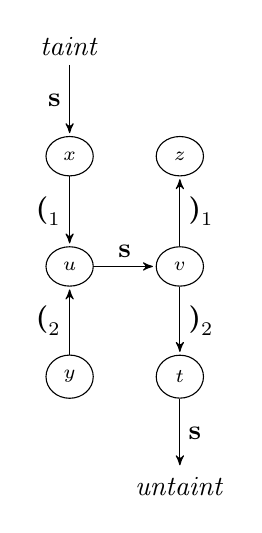
\begin{tikzpicture}[shorten >=1pt, >=stealth', node distance=1.4cm,on grid,auto]
\tikzstyle{none} = [draw=none, minimum height=0.4cm, minimum width=1cm]
   \node[none]  (a)              {\emph{taint}};
   \node[state] (b) [below of=a] {$x$};
   \node[state] (d) [below of=b] {$u$};
   \node[state] (c) [below of=d] {$y$};
   \node[state] (e) [right of=d] {$v$};
   \node[state] (f) [above of=e] {$z$};
   \node[state] (g) [below of=e] {$t$};
   \node[none]  (h) [below of=g] {\emph{untaint}};
   \path[->]
    (a) edge[horiz] node[left]  {s} (b)
    (b) edge[horiz] node[left]  {$\boldsymbol{(}_1$} (d)
    (c) edge[horiz] node        {$\boldsymbol{(}_2$} (d)
    (d) edge[horiz] node        {s} (e)
    (e) edge[horiz] node[right] {$\boldsymbol{)}_1$} (f)
    (e) edge[horiz] node        {$\boldsymbol{)}_2$} (g)
    (g) edge[horiz] node        {s} (h)

    ;    
\end{tikzpicture}

\end{multicols}

\end{posterbox}

\headerbox {Problem}{name=problem,column=3,row=0, span=6, bottomaligned=appSA}{
\begin{center} 
Find paths which satisfy constraints in form of a formal language
\end{center}

\vspace{0.4cm}

\begin{minipage}[m]{0.42\linewidth}
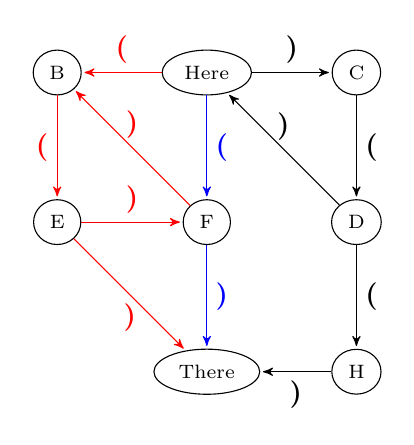
\begin{tikzpicture}[shorten >=1pt, >=stealth', node distance=1.9cm,on grid,auto]
%\tikzstyle{point} = [circle, minimum width = 3pt, fill]
   \node[state] (a) {Here};
   \node[state] (b) [left=of a] {B};
   \node[state] (c) [right=of a] {C};
   \node[state] (d) [below=of c] {D};
   \node[state] (e) [below=of b] {E};
   \node[state] (f) [below=of a] {F};
   \node[state] (g) [below=of f] {There};
   \node[state] (h) [below=of d] {H};
   \path[->]
    (a) edge[red, horiz] node[above] {(} (b)
    (a) edge[horiz] node        {)} (c)
    (a) edge[horiz, blue] node        {(} (f)
    (b) edge[horiz, red] node[left]  {(} (e)
    (c) edge[horiz] node        {(} (d)
    (d) edge[horiz] node        {(} (h)
    (d) edge[horiz] node[above] {)} (a)
    (e) edge[horiz, red] node        {)} (f)
    (e) edge[horiz, red] node[below] {)} (g)
    (f) edge[horiz, red] node[above] {)} (b)
    (f) edge[horiz, blue] node        {)} (g)
    (h) edge[horiz] node        {)} (g);    
\end{tikzpicture}
\end{minipage}\hfill
\begin{minipage}[m]{0.52\linewidth}
    \begin{center}

    Is there a path from \textbf{Here} to \textbf{There} which is a balanced string of brackets?
    
    \bigskip 
    
    Constraints are context-free
    
    $$ S \rightarrow \varepsilon \mid \boldsymbol{(} \, S \, \boldsymbol{)} \, S $$
    \end{center}

\bigskip

\begin{center}
\textcolor{red}{\textbf{(())()}} \hspace{1cm} \textcolor{blue}{\textbf{()}} \hspace{1cm} \textbf{()()}
\end{center}
\end{minipage}
}

\headerbox {Application}{name=appDB,column=9,row=0, span=3, bottomaligned=appSA}{

\begin{center}
Querying of graph databases 

\vspace{0.4cm}

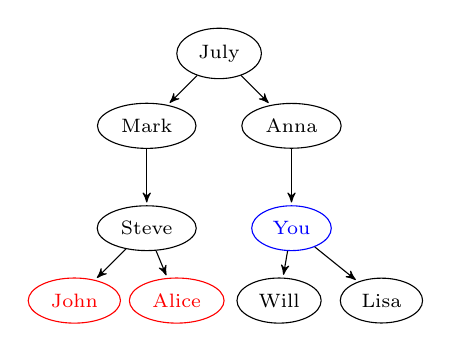
\begin{tikzpicture}[shorten >=1pt, >=stealth', node distance=1.3cm,on grid,auto]
   \node[state] (0) {July};
   \node[state] (1) [below left=of 0]  {Mark};
   \node[state] (2) [below right=of 0] {Anna};
   \node[state] (3) [below=of 1]  {Steve};
   \node[state, blue] (4) [below=of 2] {You};
   \node[state, red] (5) [below left=of 3]  {John};
   \node[state, red] (6) [below right=of 5, right=of 5] {Alice};
   \node[state] (7) [below=of 4, right=of 6] {Will};
   \node[state] (8) [below=of 4, right=of 7] {Lisa};
   
   \path[->]
%    (0) edge[horiz] node[sloped, above] {child} (1)
    (0) edge node        {} (2)
    (0) edge node        {} (1)
    (1) edge node        {} (3)
    (3) edge node        {} (5)
    (3) edge node        {} (6)
    (2) edge node        {} (4)
    (4) edge node        {} (7)
    (4) edge node        {} (8)
       ;
\end{tikzpicture}

\bigskip 

Find your cousins once removed
\begin{align*}
S& \rightarrow H \boldsymbol{\downarrow}  \\
H& \rightarrow \varepsilon \mid  \, \boldsymbol{\uparrow} \, H \, \boldsymbol{\downarrow} 
\end{align*}
\end{center}
}

    
\headerbox{Solution: Idea}{name=CFParsing,span=12,column=0,row=1,below=problem}{

%Constraints are a formal language. Searching the paths in the graph which meet the constraints is constructing a language intersection. 

%Vertices in the graph are positions in the input. Calculate parser states while traversing the graph. 

\begin{multicols}{2}

\begin{center}

\begin{center} String = linear graph \end{center} 
\begin{center}
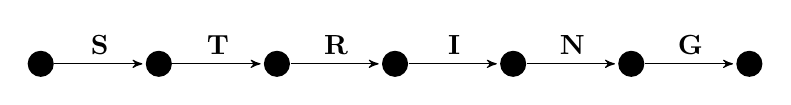
\begin{tikzpicture}[shorten >=1pt, >=stealth', node distance=1.5cm,on grid,auto]
%\tikzstyle{point} = [circle, minimum width = 5pt, fill]
   \node[point] (a) {};
   \node[point] (b)[right=of a] {};
   \node[point] (c)[right=of b] {};
   \node[point] (d)[right=of c] {};
   \node[point] (e)[right=of d] {};
   \node[point] (f)[right=of e] {};
   \node[point] (g)[right=of f] {};
   \path[->]
    (a) edge[horiz] node {S} (b)
    (b) edge[horiz] node {T} (c)
    (c) edge[horiz] node {R} (d)
    (d) edge[horiz] node {I} (e)
    (e) edge[horiz] node {N} (f)
    (f) edge[horiz] node {G} (g);
\end{tikzpicture}
\end{center}

\begin{center} Parsing = checking if the (only) path satisfies the constraints \end{center} 

\bigskip 

\bigskip 

\begin{center} What makes a graph \textbf{not} a string? \end{center}


\begin{multicols}{2}
\begin{center} Branches \end{center}

\begin{multicols}{2}
\begin{center}
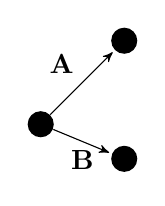
\begin{tikzpicture}[shorten >=1pt, >=stealth', node distance=1.5cm,on grid,auto]
%\tikzstyle{point} = [circle, minimum width = 3pt, fill]
   \node[point] (a) {};
   \node[point] (b)[right=of a, above right=of a] {};
   \node[point] (c)[right=of a, below=of b] {};
   \path[->]
    (a) edge[horiz] node {A} (b)
    (a) edge[horiz, below] node {B} (c);
\end{tikzpicture}

\vspace{0.4cm}

Parse along each branch 
\end{center}

\columnbreak

\begin{center}
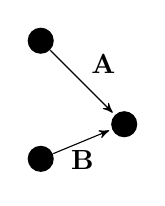
\begin{tikzpicture}[shorten >=1pt, >=stealth', node distance=1.5cm,on grid,auto]
   \node[point] (a) {};
   \node[point] (b)[left=of a, above left=of a] {};
   \node[point] (c)[left=of a, below=of b] {};
   \path[->]
    (b) edge[horiz] node {A} (a)
    (c) edge[horiz, below] node {B} (a);
\end{tikzpicture}

\vspace{0.4cm}

Merge the parsing results
\end{center}
\end{multicols}

\columnbreak 

\begin{center} Cycles 

%\end{center}
%\begin{center}
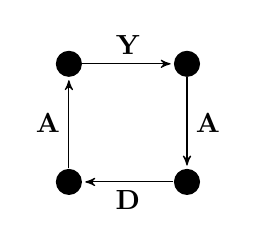
\begin{tikzpicture}[shorten >=1pt, >=stealth', node distance=1.5cm,on grid,auto]
%\tikzstyle{point} = [circle, minimum width = 3pt, fill]
   \node[point] (a) {};
   \node[point] (b)[right=of a] {};
   \node[point] (c)[below=of b] {};
   \node[point] (d)[left=of c] {};
   \path[->]
    (a) edge[horiz] node {Y} (b)
    (b) edge[horiz] node {A} (c)
    (c) edge[horiz] node {D} (d)
    (d) edge[horiz] node {A} (a);
\end{tikzpicture}

\vspace{0.2cm}

Make sure to not do 

the job twice
\end{center}
\end{multicols}
\end{center}

\columnbreak

\begin{minipage}[m]{\linewidth}

\vspace{2cm}

\begin{itemize}
  \item Each input position corresponds to a set of intermidiate parsing results
  \item Continue parsing along each branch independently
  \item Merge the sets of intermidiate results whenever two paths lead to the~same input position
  \item Continue parsing only from the \textbf{new} results
  \item Memoize the results obtained 
\end{itemize}


\end{minipage}
\end{multicols}
}

\headerbox{Generalized Parsing}
{name=sol1,column=0,span=4, row=2, below=CFParsing}
{ 
\begin{center}
Modification of the GLR and GLL algorithms 
\end{center}

\begin{multicols}{2}
\begin{center}
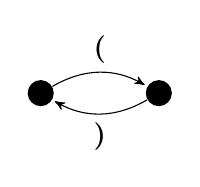
\begin{tikzpicture}[shorten >=1pt, >=stealth', node distance=1.5cm,on grid,auto]
   \node[point] (a) {};
   \node[point] (b)[right=of a] {};
   \path[->]
    (a) edge[horiz, bend left=30] node {(} (b)
    (b) edge[horiz, bend left=30] node {)} (a);
\end{tikzpicture}
\end{center}
\columnbreak
\begin{minipage}[m]{\linewidth}
\begin{align*}
S & \rightarrow \varepsilon \mid \boldsymbol{(} S \boldsymbol{)} S 
\end{align*}
\end{minipage}
\end{multicols}

\begin{center}
All derivation trees are constructed explicitly
\end{center}

\begin{center}
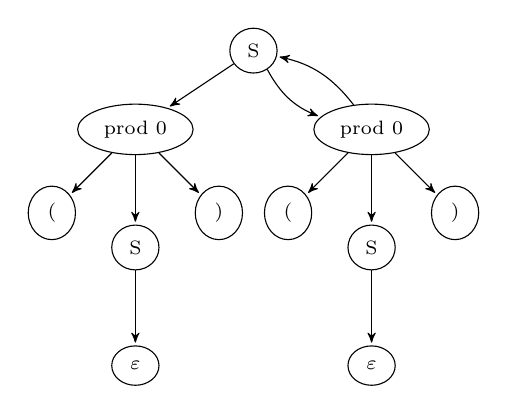
\begin{tikzpicture}[shorten >=1pt, >=stealth', node distance=1.5cm,on grid,auto]
   \node[state] (0) {S};
   \node[state] (1) [below left=1cm and 1.5cm of 0] {prod 0};
   \node[state] (2) [below right=1cm and 1.5cm of 0]  {prod 0};
   \node[state] (3) [below left=of 1]  {(};   
   \node[state] (4) [below=of 1]       {S};   
   \node[state] (5) [below right=of 1] {)};         
   \node[state] (6) [below left=of 2]  {(};   
   \node[state] (7) [below=of 2]       {S};   
   \node[state] (8) [below right=of 2] {)};
   \node[state] (9) [below=of 4]       {$\varepsilon$};   
   \node[state] (10)[below=of 7]       {$\varepsilon$};   

   \path[->]
    (0) edge[horiz              ] node {} (1)
    (0) edge[horiz,bend right=20] node {} (2)
    (1) edge[horiz              ] node {} (3)
    (1) edge[horiz              ] node {} (4)
    (1) edge[horiz              ] node {} (5)
    (2) edge[horiz              ] node {} (6)
    (2) edge[horiz              ] node {} (7)
    (2) edge[horiz              ] node {} (8)
    (2) edge[horiz,bend right=20] node {} (0)
    (4) edge[horiz              ] node {} (9)
    (7) edge[horiz              ] node {} (10)    
    ;
\end{tikzpicture}
\end{center}

}

\begin{posterbox}[name=sol2,column=4,row=4, span=4, below=CFParsing, bottomaligned=sol1]{Parser Combinators}

\begin{center}
CPS Parser Combinators with memoization
\end{center}

\lstset{language=Scala}

\begin{lstlisting}
val Query: Nonterminal
= syn ("Here" ~ S ~ "There")

val S: Nonterminal
= syn(sameGen(List(("(", ")")))

def sameGen(brs) =
  reduceChoice(
    brs.map {case (lbr, rbr) =>
      lbr ~ 
      syn(sameGen(brs).?) ~ 
      rbr
    }
  )
\end{lstlisting}

\begin{center}
Common query patterns can be written as parser combinators and reused
\end{center}
\end{posterbox}

\headerbox {Matrix Multiplication}
{name=sol3,column=8,span=4, row=2, below=CFParsing,bottomaligned=sol2}
{ 

\begin{center}
Transitive closure of a special matrix

\medskip

$T$ --- adjacency matrix

The grammar in the normal form

\begin{align*} 
T_{ij} &=\{ N \mid N \xRightarrow[]{*} \omega,  \omega \text{ path bw } i \text{ and } j \} \\
T_{ik} \times T_{kj} &= \{ A \mid B \in T_{ik}, C \in T_{kj}, A \rightarrow B C \} \\
T^{(i)} &= T^{(i-1)} \cup (T^{(i-1)} \times T^{(i-1)})
\end{align*}

\medskip

\begin{minipage}[m]{\linewidth}
\[
\begin{pmatrix}
	\{S\}     & \{A\}       & \varnothing & \{B, S\}    \\
	\{S\}       & \varnothing & \{A\}       & \{S\}     \\
	\{A, S\}  & \varnothing & \varnothing & \{S\} \\
	\{B\}       & \varnothing & \varnothing & \varnothing \\
\end{pmatrix}
\]
\end{minipage}

\bigskip

Easy to run in parallel environments: 

GPUs, multithreaded CPUs, clusters

\medskip

Any matrix multiplication library can be used
\end{center}
}

%----------------------------------------------------------------------------------------
%   REFERENCES
%----------------------------------------------------------------------------------------

%\headerbox {References}
%{name=app2,column=2,span=2, below=CFParsing}
%{
%\smaller % Reduce the font size in this block
%\renewcommand{\section}[2]{\vskip 0.05em} % Get rid of the default "References" section title
%%\nocite{*} % Insert publications even if they are not cited in the poster
%
%\bibliographystyle{unsrt}
%%\bibliographystyle{IEEEtran}
%\bibliography{biblio} % Use biblio.bib as the bibliography file
%}




    
\headerbox {\smaller{Contact us}}{name=contact,column=0,span=4,below=sol1}{
\scriptsize
Everything is available on GitHub: 

\footnotesize{https://github.com/YaccConstructor}
}

\headerbox {\smaller{Acknowledgments}}{name=ack,column=0,span=4,below=contact}{
\scriptsize
The research is supported by the JetBrains Research grant and the~Russian Science Foundation grant 18-11-00100.
}

\headerbox{\smaller{References}}{name=references,column=4,span=8,below=sol1, bottomaligned=ack}{
	
	\scriptsize % Reduce the font size in this block
	\renewcommand{\section}[2]{\vskip 0.05em} % Get rid of the default "References" section title
	\nocite{*} % Insert publications even if they are not cited in the poster
	\bibliographystyle{unsrt}
	\bibliographystyle{IEEEtran}
	\bibliography{biblio} % Use biblio.bib as the bibliography file
}
\end{poster}


\end{document}
